%\nonstopmode
\hbadness=100000
\documentclass[a4paper, 12pt]{article}
\usepackage{verbatim,amsmath,graphicx,geometry,textcomp,url}
\geometry{ a4paper, total={170mm,257mm}, left=20mm, top=20mm}

\usepackage[toc, page]{appendix}
\usepackage[dvipsnames]{xcolor}
\definecolor{subr}{rgb}{0.8, 0.33, 0.0}
\definecolor{func}{rgb}{0.76, 0.6, 0.42}

\begin{document}
\begin{center}
FORTRAN 77 Accompanying Report					\\
Ocean Wong (Hoi Yeung Wong)						\\
MSc Physics and Technology of Nuclear Reactors	\\
2018-12-25										\\
\end{center}

\section{Formulation of the problem}
A flux profile of constant spacing is provided by the user. This represents the variation of neutron flux across the entire height of the reactor.\\
The power ($P$) produced per unit volume ($V$) of fuel is then given as
\begin{align}
\frac{P}{V} &=  Q F  							\label{FirstEq} \\
\frac{P}{V} =q''' &= Q \Sigma_f^F \phi(z)						\\
  &= Q N_d \sigma_f \phi(z) 						\\
  &= Q E \frac{N_A \:\rho}{A} \sigma_f \phi(z) \label{ExpandedQ'''}
\end{align}
where the symbols has their usual meaning in nuclear engineering, but can also be found in Table \ref{table1}.
All of the above constants are computed in SI units.

At thermal equilibrium, the temperature of the coolant must monotonically increase as it travels up the cooling channels; and the rate of increase of temperature must be proportional to the power produced by that particular section fuel pin between $z$ and $z+\Delta z$, which in turn is proportional to the flux at $z$. This is given by equation \ref{IntTcool}.
\begin{align}
	T_{cool}(z)=\int\limits_{0}^{z} \frac{A_f q'''(z')}{\dot{m}C_p} dz'
	\label{IntTcool}
\end{align}
The temperature profile inside the fuel pin can then be inferred from the coolant temperature using equation \ref{Tclado} onwards.

A program is needs to be written; the aim of this program is to find out this vertical temperature profile for the coolant, exterior of the cladding, and the maximum temperature of the fuel (closest to the centre point), print them to screen and save to file.

\subsection{simplifications and justification}
The material characterstics (dimension of the reactor, Macroscopic cross-section of the fuel and other heat transfer constants) is assumed to remain constant with respect to temperature varaiation.\\

This the error contribution from this assumption is expected to be relatively small, and and using this assumption reduces the complexity of the program significantly, so that the source code is more easily understood by other programmers, and it is less likely to make a mistake.

The temperature variation is found using summation instead of integrating over the interpolated flux profile. (See Figure \ref{OnlyPicture} and equation \ref{IntTcool})\\

Finally, as a disambiguation, the flux profile provided by the user is assumed to span the entire height of the reactor, 0 to $z_{max}$, inclusive of the boundary, so that the size must be 
And therefore it must have the o	
\begin{figure}[!h]
\centering
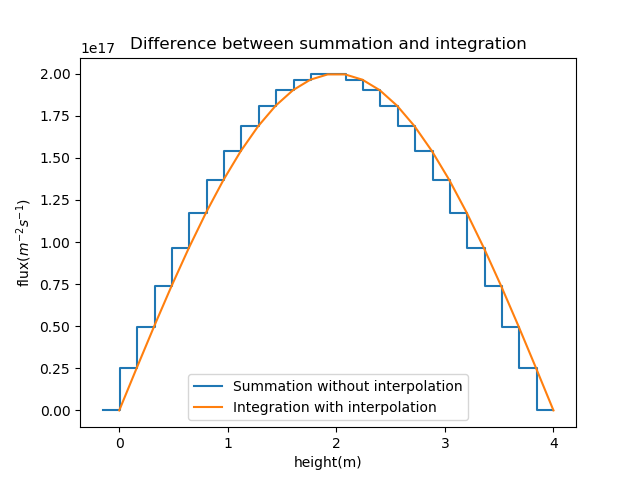
\includegraphics[height=8cm]{SumVsInt.png}
\caption{The summation approach given by equation \ref{Tcool} is identical to dividing the flux profile into steps before integrating (equation \ref{IntTcool} to find its effect on the temperature profile.}\label{OnlyPicture}
\end{figure}

The error contribution from this simplification decreases as the number of flux values provided by the user increase (the spacing decreases).

\section{Approarch}
The program is modularized using \textcolor{subr}{SUBROUTINE}s and \textcolor{func}{FUNCTION}s. The layout is as follows:\\

After printing some preliminary information about the program (authorship and purpose),
\begin{itemize}
	\item \texttt{\textcolor{subr}{PrintProgramHeader}()}
\end{itemize}

it prompts for an input of the file name (which has to be in the same directory as the executable .out file) from the user.
\begin{itemize}
	\item \texttt{\textcolor{subr}{GetFileName}(fileName)}
	\item \texttt{\textcolor{subr}{ScanFlux}(fileName, length, flux, arysize)}
\end{itemize}
(The program will exit if the file can be opened but cannot be read as floating point values, such that the user can change the content of the input file and re-run the program.)\\
The values read from the file are stored in an array (of size 1023) in the main program. \\
This sets an upper limit of 1023 to the number of values that can be provided by the input file (and therefore limits the spatial resolution in vertical flux profile).\\

%Initizlise parameters
After ensuring that the file exist and is read without error, the function \texttt{Init\_params} prompts for the reactor type from the user, such that the proper parameters for the reactor can be chosen.
\begin{itemize}
	\item \texttt{\textcolor{func}{Init\_params}(length)} 
	\begin{itemize}
		\item \texttt{\textcolor{func}{GetReactorType}()} 
		\item \texttt{\textcolor{subr}{AGRparameters}($z_{max}$,$\dot{m}$,$C_p$,$h_c$,$T_{in}$,$E$,$d_f$,$d_h$,$T_c$,$k_c$,$h_g$)}
		\item \texttt{\textcolor{subr}{PWRparameters}($z_{max}$,$\dot{m}$,$C_p$,$h_c$,$T_{in}$,$E$,$d_f$,$d_h$,$T_c$,$k_c$,$h_g$)}
		\item \texttt{\textcolor{subr}{UO2MaterialConstants}(k\_f,Macroscopic,Q,E)}
	\end{itemize}
\end{itemize}
The parameters are then saved in \texttt{\textcolor{red}{COMMON}} blocks to be shared with other subroutines below.\\
The number of flux values read from the input file (which is stored as the variable \texttt{length}) is needed to determine how many steps to divide the height of the reactor \texttt{z} into; and level of enrichment is required to calculate the Macroscopic cross-section for fission of the fuel.\\


%Make file name
The program then appends \texttt{"\_T\_output"} after the input file's name as the output file.
\begin{itemize}
	\item \texttt{\textcolor{func}{OutFileName}(fileName)} 
\end{itemize}
(i.e. if the input file is \texttt{flux.txt}, then the output file will be named \texttt{flux\_T\_output.txt}.) \\
If a file of the same name as the output file already exist, an option is given to the user to either proceed to overwrite the file or stop the program, to prevent silent overwriting.\\
%Explanation of the size of the arrays due to the looping behaviour.

%Do loop
The temperature at each height is then calculated using a \texttt{DO} loop, looping over all actively used values of flux.
\begin{itemize}
	\item[]
	\begin{itemize}
	\item \texttt{\textcolor{subr}{IncrementHeight}(z,z1)}
	\end  {itemize}
\end  {itemize}

If there are only 101 values in the input file \texttt{flux.txt}, then it will only loop over the first 101 elements in each array, with the exception of the two arrays \texttt{z} and \texttt{Tcool}, which will loop over the first 102 values of the arrays. \\
This is because the subroutines for calculating the values of each element in these two arrays propagates the value upwards(calculates \texttt{var1(i+1)} from \texttt{var1(i)}) instead of laterally (calculates \texttt{var2(i)} from \texttt{var1(i)}).\\
Therefore the sizes of these two arrays are of \texttt{arysize+1}=1024 to account of the edge case where \texttt{length}==\texttt{arysize}\\

The corresponding temperature changes can then be calculated using these information.
Since the term $\frac{A_f q'''(z)}{\pi}$ (where q''' is a z-dependent variable given by equation \ref{ExpandedQ'''}) appears in every one of the equations,
\begin{align}
\frac{A_f q'''}{\pi} = (d_f^2-d_h^2) Q E \frac{N_A \:\rho}{A} \sigma_f \phi(z) \label{Afq'''pi}
\end{align}
an array \texttt{q\_lin\_over\_pi} is allocated to store its values. It is named as such because $q''' A_f = q'$ which is the linear heat generation rate, i.e. heat produced per unit length of fuel pin:
\begin{itemize}
	\item[]
	\begin{itemize}
	\item \texttt{\textcolor{subr}{LinearHeatGenOverPi}(flux(i), q\_lin\_over\_pi(i))}
	\end  {itemize}
\end  {itemize}
This, and the following subroutines, retrieve parameters for the reactor via common blocks. The definition of these parameters are listed in Table \ref{table2}.\\

The coolant temperature is then 
\begin{align}\label{Tcool}
T_{cool}(z+\Delta z)= T_{cool}(z)+ \bigg(\frac{A_f q'''(z)}{\pi}\bigg) \pi \frac{\Delta z}{\dot{m}C_p}
\end{align}
which is calculated by the following subroutine using \texttt{\textcolor{red}{COMMON /Tcool/ dz, mdot, Cp}}

A better approach is to take the average of the flux at $z$ and $z+\Delta z$
	
\begin{align}
T_{cool}(z+\Delta z)= T_{cool}(z)+ \bigg(\frac{\big(\frac{A_f q'''(z+\Delta z)}{\pi}\big)+\big(\frac{A_f q'''(z)}{\pi}\big)}{2}\bigg) \pi \frac{\Delta z}{\dot{m}C_p}
\label{LinearInterp}
\end{align}
This more accurately represents the temperature change of the coolant after travelling from $z$ to $\Delta z$; but to keep the program simple the former option was adopted, leading to the result:

\begin{itemize}
	\item[]
	\begin{itemize}
	\item \texttt{\textcolor{subr}{HeatCoolant}(Ti,Ti1,qi)}
	\end{itemize}
\end{itemize}

In a similar vein, the equation for calculating the temperature of various components and the associated subroutines to do the computation are listed below:

Exterior of cladding:
\begin{align}
T_{oc}(z)=T_{cool}(z)+ \bigg(\frac{A_f q'''(z)}{\pi}\bigg) \frac{1}{h_c d_c} \label{Tclado}
\end{align}
calculated by the following subroutine with the aid of \texttt{ \textcolor{red}{COMMON /Toc/   hc, dc} }
\begin{itemize}
	\item[]
	\begin{itemize}
	\item \texttt{\textcolor{subr}{CoolCladding}(   Tcool(i),Tclado(i),q\_lin\_over\_pi(i))}
	\end  {itemize}
\end  {itemize}

Interior of cladding:
\begin{align}
T_{ic}(z) = T_{oc}(z) + \bigg(\frac{A_f q'''(z)}{\pi}\bigg) \frac{1}{2 k_c} ln\bigg(\frac{d_c}{d_f}\bigg) \label{Tcladi}
\end{align}
calculated by the following subroutine with the aid of \texttt{ \textcolor{red} {COMMON /Tic/   kc, ln\_d\_c\_over\_d\_f} }
\begin{itemize}
	\item[]
	\begin{itemize}
	\item \texttt{\textcolor{subr}{CoolCladdingIn}(Tclado(i),Tcladi(i),q\_lin\_over\_pi(i))}
	\end  {itemize}
\end  {itemize}

Surface of fuel pellets:
\begin{align}
T_{fo}(z) = T_{ic}(z) + \bigg(\frac{A_f q'''(z)}{\pi}\bigg) \frac{1}{h_g d_f}
\label{Tfuelo}
\end{align}
calculated by the following subroutine with the aid of \texttt{ \textcolor{red} {COMMON /Tof/   hg, df} }
\begin{itemize}
	\item[]
	\begin{itemize}
	\item \texttt{\textcolor{subr}{CoolFuel}(      Tcladi(i),Tfuelo(i),q\_lin\_over\_pi(i))}
	\end  {itemize}
\end  {itemize}

Maximum temperature inside fuel (nearest to the centre):
\begin{align}
T_{fmax}(z) = T_{of}(z)+ \bigg(\frac{A_f q'''(z)}{\pi}\bigg) \frac{1}{4 k_f}  
- \bigg(\frac{A_f q'''(z)}{\pi}\bigg) \frac{1}{2 k_f} \frac{d_h^2}{d_f^2-d_h^2} ln\bigg(\frac{d_f}{d_h}\bigg)\label{Tfmax}
\end{align}
where the last term $\rightarrow 0$  as $d_h\rightarrow 0$,
calculated by the following subroutine with the aid of \texttt{ \textcolor{red} {COMMON /Tfmax/ kf, dh2\_df2\_dh2\_ln\_df\_dh} }
\begin{itemize}
	\item[]
	\begin{itemize}
	\item \texttt{\textcolor{subr}{FindHottest}(   Tfuelo(i), Tfmax(i),q\_lin\_over\_pi(i))}
	\end  {itemize}
\end  {itemize}

The values of interest are printed to the screen as well as into the file as an extra line:
\begin{itemize}
	\item[]
	\begin{itemize}
	\item \texttt{\textcolor{subr}{SaveTemps}(z(i), Tcool(i),Tclado(i),Tfmax(i), o     )}
	\end  {itemize}
\end  {itemize}

\ \\
After looping through all values, the file is closed, and the end time of the program is printed,
\begin{itemize}
	\item \texttt{\textcolor{subr}{finished}()}
\end{itemize}
and the program is exited.

%Section on ERROR HANDLING______________________________________________________________
\section{Error handling features}
The program may encounter user induced error in 4 locations:
\begin{enumerate}
	\item Prompting the user to input the file name (user input)
	\item Reading the file
	\begin{enumerate}
		\item If file contains unreadable lines
		\item If file size is too big
	\end{enumerate}
	\item Prompting the user to input the reactor type.
	\item Saving the output file
\end  {enumerate}

Which are handled as follows:
\begin{enumerate}
	\item Check that file exist; if not, prompt user to type in the file name again (loop infinitely until a correct file name is found)
	\item Exit the main program after:
	\begin{enumerate}
		\item printing the line number where there is an unrecognized character.
		\item Print the size of the allocated memory, and printing the line number where memory overflow will occur.
	\end{enumerate}
	\item Check that the input is correct, if not ask user to try again (loop infinitely)
	\item If file exist, warn user and ask user whether to overwrite or not
	\begin{enumerate}
		\item if 'y', resume to overwrite the old file with the new outputs.
		\item if 'n', exit the program
	\end{enumerate}
\end  {enumerate}

\section{Portability of source code onto other machines}
This program was written on a Linux (Ubuntu 18.04.1 LTS) machine compiled by gfortran. It has been subsequently been tested again on a Scientific Linux 7.3 (Nitrogen).

This source is expected to work across multiple platforms since:
\begin{itemize}
	\item Despite the use of many subroutines and functions, they are all kept in the same file, so the source code can be compiled on its own without dependance on other files/libraries.
	\item No local file paths were specified
	\item No special line ending (e.g. \textbackslash r\textbackslash t) were used.
	\item The source code is written in FORTRAN 77 syntax, so it should be compilable on most platforms by any currently actively maintained FORTRAN compilers. (e.g. GFortran, which is available on macOS and Windows as well)
\end{itemize}

\section{Potential future improvements}
Currently the program takes \emph{any} flux values, and calculate an output temperature, without checking whether these flux values are reasonable or not.

%Improving accuracy
The program makes some assumption about the material, i.e. it has temperature independent density, and the doppler coefficient =0. In a real reactor, the fuel should expand and be less susceptible to fission by thermal neutrons, so this should be taken into account in a more advanced version of the program.

%Checking that numbers are sensible
A more advanced version of this program may check for negative values in the input file's flux values, which is unphysical. And if the appropriate data is found, such as the recrystallization temperature of the cladding, and safe operating temperature of UO2, the safe operating conditions can be found, so that the program can print a warning when the temperature goes over the safe limits.

%Header
This program also exit upon encountering any non-floating point value lines. In the future, if one wishes to, this program can be improved upon by adding a functionality to skip over lines starting with "\#", which typically denotes a header.

%Memory restriction
It is also restricted to read a file below a certain size, arbitrarily chosen as 1023. This restriction can be lifted using some of the more recent FORTRAN syntax, e.g. with automatic object in later versions of FORTRAN, or with other language (e.g. Python). However, this is very difficult to achieve with FORTRAN 77, as size of the array needs to be known before any file reading operation begins. So while this limit can be easily edited in the source code (by editing the parameter \texttt{arysize}), this value will be fixed once the code is compiled.
\cite{AutoObj}

%Summation-> Integration
Lastly, this program uses simple summation of the given flux value over the intervals of height. In the future, cubic spline can be used to obtain the flux value at any arbitrary height between any two data points; and then an integration over that can be carried out, such that the temperature profile can still be well approximated even when very few data points are provided by the user, increasing the ease of use.

\newpage
\begin{appendices} 
	
\begin{table}[h!b]
\begin{tabular}{llll}
\hline
symbol&name in&physical meaning & SI unit\\
&program&&\\
\hline
\hline
$F$		&& reaction(fission) rate per volume							&$m^{-3}s^{-1}$\\
$Q$ 	&\texttt{Q}&Q value of the reaction 											&J(Joule)\\
$\phi(z)$&\texttt{flux(i)}& 2200 ms${}^{-1}$ flux (thermal neutron flux) as a function of height &$m^{-2}s^{-1}$\\
$\Sigma_f^F$&\texttt{Sigma\_mac}& macroscopic fission cross section of the fuel (UO${}_2$)		&$m^{-1}$\\
&/\texttt{Macroscopic}&&\\
$N_d$ 	&& number density of ${}^{235}$U 									&$m^{-3}$\\
$\sigma_f$&\texttt{sigma\_mic}& microscopic fission cross section of UO${}_2$	&$m^{2}$\\
&&&=$10^{28}$barns\\
$\rho $ &\texttt{rho}& density of UO${}_2$											&kg$m^{-3}$\\
$E$ 	&\texttt{E}& enrichment (fraction of ${}^{235}$U)								&1\\
$A$ 	&\texttt{A}& molar mass of UO${}_2$(dependent on enrichment)					&kg\\
\hline
\end{tabular}
\caption{Definitions of constants used in equation \ref{FirstEq} to \ref{ExpandedQ'''} }\label{table1}
\end{table}

\begin{table}[h!b]
\begin{tabular}{llll}

\hline
symbol&name in program&physical meaning & SI unit\\
\hline
$z_{max}$&\texttt{zmax}&Total height of channel 				&m\\
$\dot{m}$&\texttt{mdot}&Mass flow rate per channel 		&$kgs^{-1}$ \\
$C_p$	&\texttt{Cp}&Specific heat capacity of coolant 		&$Jkg^{-1}$ $K^{-1}$ \\
$h_c$	&\texttt{hc}&Convective heat transfer coefficient&W$m^{-2}$ $K^{-1}$ \\
$T_{in}$&\texttt{Tin}&Inlet coolant temperature 			& \textdegree C\\
\hline
$d_f$	&\texttt{df}&Outer diameter of fuel pellet, &m\\
$d_h$	&\texttt{dh}&Inner diameter of fuel pellet, &m\\
\hline
$t_c$	&\texttt{Tc}&Thickness of cladding &m\\
$k_c$	&\texttt{kc}&Thermal conductivity of cladding,  &$Wm^{-1}$ $K^{-1}$ \\
$h_g$	&\texttt{hg}&Gap conductance, h g &W$m^{-2}$ $K^{-1}$ \\
\hline
$d_c$	&\texttt{dc}&Outer diameter of cladding&m\\
\hline

\end{tabular}
\caption{Definitions of constants used from equation \ref{Afq'''pi} to \ref{Tfmax}}\label{table2}
\end{table}

\end{appendices}

\begin{thebibliography}{1}
\bibitem{AutoObj}
Ibm.com. (2018). IBM Knowledge Center. [online] Available at: \url{https://www.ibm.com/support/knowledgecenter/SSGH4D_13.1.0/com.ibm.xlf131.aix.doc/language_ref/autoobj.html} [Accessed 26 Dec. 2018].
\end  {thebibliography}

%No matter how many references I have, it is NOT worth it to make a .bib file.

\end{document}